\documentclass[a4paper,12pt]{article} 
\sloppy

% report, book

% Рисунки
\usepackage{graphicx}
\DeclareGraphicsExtensions{.pdf,.png,.jpg}
\usepackage{wrapfig}
% Гиперссылки
\usepackage{hyperref}
\usepackage[rgb]{xcolor}
\hypersetup{
    colorlinks=true,
	urlcolor=blue,
    unicode=true
}

%  Русский язык

\usepackage[T2A]{fontenc} % кодировка
\usepackage[utf8]{inputenc} % кодировка исходного текста
\usepackage[english,russian]{babel}	% локализация и переносы
\usepackage {indentfirst} % отступ
\usepackage[left=2.5cm,right=2.5cm,
    top=2cm,bottom=2cm,bindingoffset=0cm]{geometry}

% Кавычки
\usepackage {csquotes}
\DeclareQuoteStyle{russian}
    {\guillemotleft}{\guillemotright}[0.025em]
    {\quotedblbase}{\textquotedblleft}
\ExecuteQuoteOptions{style=russian}

% Код
\usepackage {listings}
\lstset{tabsize=2,
    breaklines,
    columns=fullflexible,
    flexiblecolumns,
    numbers=left,
    numberstyle={\footnotesize},
    extendedchars}


% Математика
\usepackage{amsmath,amsfonts,amssymb,amsthm,mathtools} 
\usepackage{biblatex}
\addbibresource{biblio.bib}



\usepackage{wasysym}
\begin{document} 
\title{Временная фильтрация изображений. HDR+}
\author{Андрей Алексеев}
\maketitle

\section{Введение}
Съемка при недостаточном освещении всегда являлась проблемой для фотографов и задачей, которую решают инженеры. Если затвор открыт на слишком короткое время, то из-за недостатка падающих фотонов, тепловой шум начинает доминировать на изображении. Но если оставить затвор фотокамеры открытым надолго, то это не спасет от теплового шума, ведь матрица камеры будет нагреваться и шум станет более заметным. К тому же, чтобы снимать несмазанные изображения на длинной выдержке нужно использовать штатив или, по крайней мере, монопод. Конечно, можно увеличить светочувствительность матрицы (ISO), но это тоже не спасет от шума на изображении.


\section{Различные способы борьбы с шумом в условиях недостаточного освещения}
В профессиональных цифровых камерах инженеры предложили увеличить размер каждого пикселя в матрице. Такой подход отлично работает в дорогих и больших фотоаппаратах. Но для массового потребления он не подходит. Матрицы в телефонах очень маленькие, а значит и размер каждого пикселя в несколько раз меньше, чем в большом фотоаппарате.

Тогда можно воспользоваться программной обработкой изображений. И самый первый и все еще самый популярный алгоритм, который появился в смартфонах -- это HDR (High Dynamic Range). При съемке фотографии, телефон делает несколько снимков (обычно от 3 до 5) с разной выдержкой, чтобы уловить детали в светлой части изображения и в темной части изображения, как на рисунке \ref{fig:shutter}. Затем эти фотографии объединяются в одну по некоторому алгоритму, который обычно учитывает сдвиг и яркость на разных участках изображения \cite{Habr1}.

\begin{figure}[h]
\centering
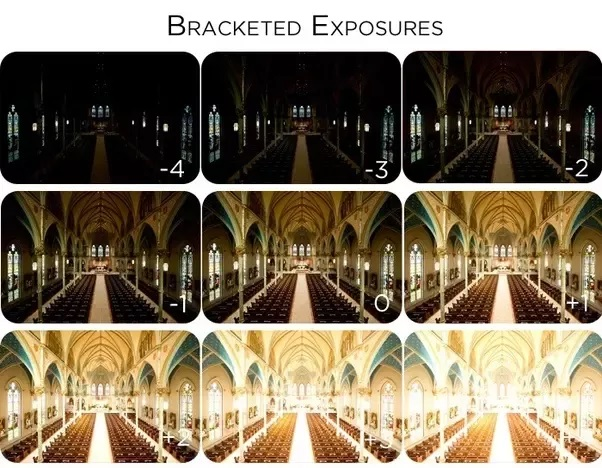
\includegraphics[width=0.7\linewidth]{shutter_speed.jpg}
\caption{Изображения с различной выдержкой}
\label{fig:shutter}
\end{figure}

Тем не менее использование HDR может приводить к нежелательным эффектам, таким как на рисунке \ref{fig:HDR_cons}

\begin{figure}[h!]
\centering
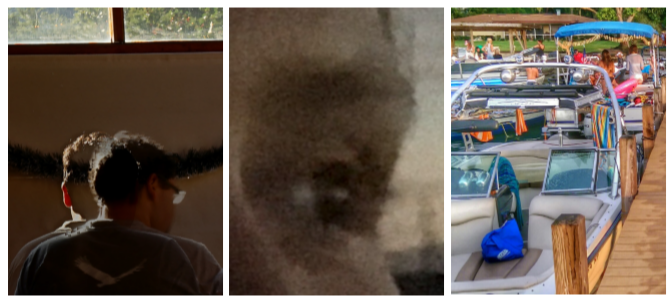
\includegraphics[width=0.7\linewidth]{HDR.png}
\caption{Ошибки HDR: <<призрачное>> изображение, излишняя работа алгоритма шумоподавления и излишнее сжатие цветового простанства}
\label{fig:HDR_cons}
\end{figure}

\section{Современный подход}
Сразу несколько исследований сфокусировались на задаче улучшения фотографий со смартфона в условиях недостаточного освещения \cite{Gavic, Google2}. В обеих статьях также предлагается делать несколько изображений для их последующего объединения, только теперь эти изображения делаются с одинаковой выдержкой. Также в алгоритме Google оценивается экспозиция снимаемой сцены, и если динамический диапазон изображения довольно широкий, то также применяется данный алгоритм, который был назван HDR+. В \cite{Google2} предлагается использовать гистограмму для оценки переэкспонированных пикселей и недоэкспонированных пикселей, причем алгоритм пытается максимально уменьшить количество переэкспонированных пикселей, тогда как темные участки изображения воcстановятся при объединении снимков. 

Для верного выставления экспозиции в различных сценах был обучен алгоритм, который способен распознавать эти самые сцены и настраивать экспозицию, выдержку и ISO для того, чтобы передать натуральные цвета на изображении. 

Также в составе HDR+ работает алгоритм, который оценивает освещенность сцены: если сцена яркая, то для получения изображения достаточно 2 снимков, для темных сцен может быть необходимо до 8 снимков.

Несмотря на то, что существуют более точные алгоритмы соединения снимков, исследователи Google говорят об их вычислительной сложности и используют $L_2$-норму по отдельным частям изображения в HDR+. Этот метод работает не идеально точно, но способен найти общие регионы на двух изображениях. Непосредственное же объединение снимков в один и фильтрация шума происходят уже на следующем шаге. Для начала выбирается опорное изображение \cite{Google1,Wiki1}. Затем от каждого изображения берется его пространственный Фурье образ и объединяется с опорным по формуле \ref{sum}

\begin{equation}
\label{sum}
    \hat{T_0} = - \frac{1}{N} \sum\limits_{i=0}^{N-1} T_i(\omega) + A_i(\omega)[T_0(\omega) - T_i(\omega)],
\end{equation}
где $T_i(\omega)$ - это Фурье образ частоты $\omega$, полученный из i-го изображения. А $A_i(\omega)$ - коэффициент, который отвечает за степень совмещения опорного изображения и i-го (\ref{A}).

\begin{equation}
\label{A}
    A_i(\omega) = - \frac{|T_0(\omega) - T_i(\omega)|^2}{|T_0(\omega) - T_i(\omega)|^2 + c\sigma^2},
\end{equation}
где $\sigma^2$ -- дисперсия шума, которая оценивается по модели шума для каждой частоты. 
Востановление цветов на полученном изображении происходит по алгоритму \cite{46440}.


\printbibliography[heading=bibintoc]
\end{document}
